%\documentclass[12pt]{article}
%\usepackage[a4paper, margin=1in]{geometry} 
%\usepackage{graphicx} 
%\usepackage{hyperref}
%\usepackage{float}
%\usepackage{multicol}
%\usepackage{multirow}
%\usepackage[font=small, labelfont=bf]{caption}
%
%\begin{document} 

%
% Lookup table of matching n-grams
%
\subsection{Lookup table of matching n-grams}
A lookup table can be used for effectively finding n-gram matches.

%
% Terminology
%
\subsubsection*{Terminology} 
\begin{itemize}
\item Indices: positions in q
\item Matching n-grams: Possible matching n-grams by threshold score $T$
\end{itemize}

%
% Example of creating a lookup table
%
\subsubsection*{Example of creating a lookup table} 

\begin{multicols}{2}
\begin{verbatim}
    q: ACGTAC 
    2-gram: AC, CG, GT, TA, AC
    T: 3
\end{verbatim}
\vfill\null
\columnbreak

Score matrix:
\begin{figure}[H]
      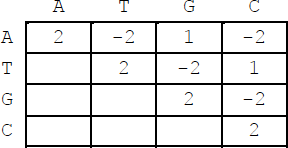
\includegraphics[width=0.25\textwidth]{fig05/score_matrix.png}
\end{figure}

\end{multicols} 

\medskip  

%
% 1. Index of q
%
\subsubsection*{Step 1. Index of q} 
Add indices to all n-grams.

\begin{table}[h]
\small
\begin{tabular}{|l|l|}
\hline
\textbf{Index} & \textbf{N-gram} \\ \hline
1              & AC              \\ \hline
2              & CG              \\ \hline
3              & GT              \\ \hline
4              & TA              \\ \hline
5              & AC              \\ \hline
\end{tabular}
\end{table}


%
% 2. Scores of segment pairs and matching n-grams
%
\subsubsection*{Step 2. Scores of segment pairs and matching n-grams} 

Calculate scores between the first n-gram AC and all its matching n-grams.
\begin{table}[H]
\small
\begin{tabular}{|l|l|l|}
\hline
\textbf{N-gram} & \textbf{Matching n-gram} & \textbf{Score} \\ \hline
AC              & AA                       & $2+(-2)=0$       \\ \hline
AC              & AC                       & $2+2=4$          \\ \hline
AC              & AG                       & $2+(-2)=0$       \\ \hline
AC              & AT                       & $2+1=3$          \\ \hline
AC              & CA                       & $(-2)+(-2)=-4$   \\ \hline
AC              & CC                       & $(-2)+2=0$       \\ \hline
AC              & CG                       & $(-2)+(-2)=-4$   \\ \hline
AC              & CT                       & $(-2)+1=-1$      \\ \hline
AC              & GA                       & $1+(-2)=-1$      \\ \hline
AC              & GC                       & $1+2=3$          \\ \hline
AC              & GG                       & $1+(-2)=-1$      \\ \hline
AC              & GT                       & $1+1=2$          \\ \hline
AC              & TA                       & $(-2)+(-2)=-4$   \\ \hline
AC              & TC                       & $(-2)+2=0$       \\ \hline
AC              & TG                       & $(-2)+(-2)=-4$   \\ \hline
AC              & TT                       & $(-2)+1=-1$      \\ \hline
\end{tabular}
\end{table}

\noindent
Use threshold $T =3$.
\begin{table}[H]
\small
\begin{tabular}{|l|l|l|}
\hline
\textbf{N-gram} & \textbf{Matching n-grams} & \textbf{Scores} \\ \hline
AC              & AC, AT, GC                & 4, 3, 3         \\ \hline
\end{tabular}
\end{table}

\noindent
Repeat the same procedure for all n-grams of q and add their indices.
\begin{table}[H]
\small
\begin{tabular}{|l|l|l|l|}
\hline
\textbf{Index} & \textbf{N-gram} & \textbf{Matching n-grams} & \textbf{Scores} \\ \hline
1              & AC              & AC, AT, GC                & 4, 3, 3         \\ \hline
2              & CG              & CG, TG, CA                & 4, 3, 3         \\ \hline
3              & GT              & GT, AT, GC                & 4, 3, 3         \\ \hline
4              & TA              & TA, CA, TG                & 4, 3, 3         \\ \hline
5              & AC              & AC, GC, AT                & 4, 3, 3         \\ \hline
\end{tabular}
\end{table}

%
% 3. Lookup table of matching n-grams
%
\subsubsection*{Step 3. Lookup table of matching n-grams} 

Transform the table above to create a lookup table of matching n-grams.
\begin{table}[H]
\small
\begin{tabular}{|l|l|l|}
\hline
\textbf{Matching n-gram} & \textbf{Indices of q} & \textbf{Scores of segment pairs} \\ \hline
AC                       & 1, 5                  & 4, 4                             \\ \hline
GC                       & 1, 3, 5               & 3, 3, 3                          \\ \hline
AT                       & 1, 3, 5               & 3, 3, 3                          \\ \hline
CG                       & 2                     & 4                                \\ \hline
TG                       & 2, 4                  & 3, 3                             \\ \hline
CA                       & 2, 4                  & 3, 3                             \\ \hline
GT                       & 3                     & 4                                \\ \hline
TA                       & 4                     & 4                                \\ \hline
\end{tabular}
\end{table}

%
% 4. Search
%
\subsubsection*{Step 4. Search} 

\begin{verbatim}
    d1: AAAGTG 
    
    2 hits
    GT – index: 3, score: 4
    TG – index: (2, 4), score: (3, 3)
\end{verbatim}

%
% Exercise \thesection.1
%
\subsubsection*{Exercise \thesection.1}
Create a lookup table of 2-grams with the indices of q and the scores of segment pairs. Use the threshold $T$ and pre-calculated scores of 2-gram segment pairs.

\begin{verbatim}
    q: CATG
    T: 3
\end{verbatim}

\noindent
The table below shows pre-calculated scores of 2-gram segment pairs.
\begin{table}[H]
\small
\begin{tabular}{|l|l|l|l|}
\hline
\multirow{2}{*}{\textbf{Matching n-gram}} & \multicolumn{3}{c|}{\textbf{N-gram}}    \\ \cline{2-4} 
                                          & \textbf{CA} & \textbf{AT} & \textbf{TG} \\ \hline
AA                                        & 0           & 0           & -1          \\ \hline
AC                                        & -4          & 3           & -4          \\ \hline
AG                                        & -1          & 0           & 0           \\ \hline
AT                                        & -4          & 4           & -4          \\ \hline
CA                                        & 4           & -4          & 2           \\ \hline
CC                                        & 0           & -1          & -1          \\ \hline
CG                                        & 3           & -4          & 3           \\ \hline
CT                                        & 0           & 0           & -1          \\ \hline
GA                                        & 0           & -1          & -1          \\ \hline
GC                                        & -4          & 2           & -4          \\ \hline
GG                                        & -1          & -1          & 0           \\ \hline
GT                                        & 4           & 3           & -4          \\ \hline
TA                                        & 3           & -4          & 3           \\ \hline
TC                                        & -1          & -1          & 0           \\ \hline
TG                                        & 2           & -4          & 4           \\ \hline
TT                                        & -1          & 0           & 0           \\ \hline
\end{tabular}
\end{table}

\bigskip 

%\end{document}
